\chapter{Light statistics and photodetection}\label{chap:6-stat-props-of-light}

\section{Statistical properties of light}\label{sec:stat-props-of-light}
Classical models describe light as a continuous train of electromagnetic waves, but this is only an approximation, since real light is emitted by atoms, with a \textbf{finite lifetime}. However, this lifetime is typically much shorter than the detector integration time $\tau_D$, which means that \textbf{individual emission bursts cannot be resolved}. As a consequence, one observes a well-defined average intensity that fluctuates on timescales longer than $\tau_D$. 

We can model classical light sources as a large number of atoms emitting independently. In a gas, atoms move and produce frequency shifts, while collisions interrupt the emission process and randomize the phase, leading to phase fluctuations.

Observe that:
\begin{itemize}
    \item A light source has a finite spectral width, meaning that its frequency is not perfectly constant. It also exhibits \textbf{intensity noise}, which implies that the amplitude of the light changes in time due to fluctuations in the number of emitting atoms and to random phase jumps in the field emitted by individual atoms. These features allow us to distinguish between classical and quantum light sources;
    
    \item Studying line-shapes with spectroscopy also provides information about the energy levels of the emitting system;
    
    \item Measuring the statistical properties of light gives access to temporal noise traces, which are relevant in quantum optics, as well as to coherence and correlation functions.
\end{itemize}

If we recall the Mach-Zehnder interferometer (Fig.~\ref{1-mach-zehnder}), the interference fringes are determined by the phase difference between the beams propagating along the two optical paths. All the discussion made before assumes a stable source frequency.
\calloutwarn{If the source has a finite spectral width $\Delta\omega$, the fringes are washed out because the contributions associated with different frequencies no longer interfere with full visibility, \textbf{bright fringes} with $\omega_1$ right \textbf{overlap with dark fringes} with $\omega_2$.}

\subsection{Coherence}

We can define \textbf{coherence} as the degree of correlation of the field, and it can be spatial or temporal. In the present discussion we are interested in temporal fluctuations, which are quantified by the \textbf{coherence time} $\tau_c$, defined as the \hl{duration over which the phase of the wave train remains correlated}. In the same way, we can define the \textbf{coherence length} as
\[
L_c = c\,\tau_c.
\]

\calloutinfo{In a Mach-Zehnder interferometer, interference fringes can be observed only when the optical path difference is smaller than the coherence length $L_c$.}

\subsection{Chaotic light sources}\label{subsec:6-chaotic-light-sources}

Suppose that:
\begin{itemize}
    \item The light source is a \textbf{gas discharge lamp}, where the atoms are excited and emit radiation. The emission is determined by the spread in atomic velocities (\emph{Doppler broadening}) and by random emission events. Such a source is called a \textbf{chaotic light source}, like thermal cavities and filament lamps.
    
     \item We assume that \textbf{collision broadening dominates}, which causes elastic phase interruptions. Atoms emit trains of electromagnetic waves, but \hl{collisions shift the energy levels and interrupt the radiation emission}. After a collision, emission resumes with the same characteristics as before, but the phase is now unrelated to the previous one. 
     Let us assume that the collision time is short, so that we can neglect the radiation emitted during the collision itself.
     
    \item Suppose to assume that the \textbf{polarization is fixed} and we can focus light in order to obtain a well defined collimated beam far away from the source. 
 \end{itemize}

The total amplitude of the electric field, sum of the emission of each atom independent one to another, would be:
\begin{equation}\label{eqn:6-total-field}
\begin{split}
E_{\text{tot}}(t) &= \sum_{i=1}^{N} E_i(t) = \\[0.5ex]
&= E_0 e^{-i\omega_0 t}\sum_{i=1}^{N} e^{i\phi_i(t)} = \\[0.5ex]
&= E_0 e^{-i\omega_0 t}\, a(t)\, e^{i\phi(t)}
\end{split}
\end{equation}

where $E_0$ and $\omega_0$ are constants, while $\phi(t)$ changes over time after each collision. Here the phase angles $\phi_1,\ldots,\phi_N$ fluctuate randomly, so the corresponding phasors can be viewed as unit vectors oriented in random directions. In phase space, this can be imagined as a random-walk process.

\hl{The total field therefore consists of a wave at frequency $\omega_0$ with \textbf{random amplitude} $a(t)$ and \textbf{random phase}}.
Notice that at optical frequencies, $f\approx 10^{15}\,\text{Hz}$, the electric field varies extremely rapidly in time, so its instantaneous value is not practical to measure. It is better to perform a time average.

We now introduce the \textbf{Poynting vector} for a wave propagating along the generic direction $\hat{k}$:
\begin{equation}\label{eqn:6-generic-em-wave}
\begin{cases}
    \vec{E} = \vec{E}_0 \cos(\vec{k}\cdot\vec{r}-\omega t)\\[0.5ex]
    \vec{B} = \vec{B}_0 \cos(\vec{k}\cdot\vec{r}-\omega t)
\end{cases}
\end{equation}
\begin{equation}\label{eqn:6-poynting-vector}
\begin{split}
    \vec{S}&=\frac{1}{\mu_0}\,\vec{E}\times\vec{B}=\\[0.5ex]
    &=\varepsilon_0 c^2\,\vec{E}\times\vec{B}=
    \varepsilon_0 c^2\,\vec{E}_0\times\vec{B}_0\,
    \cos^2(\vec{k}\cdot\vec{r}-\omega t)=\\[0.5ex]
    &=\varepsilon_0 c^2 E_0 B_0 \cos^2(\vec{k}\cdot\vec{r}-\omega t) \hat{k}
\end{split}
\end{equation}

If we take the cycle average over a period $T$ of the Equation~\ref{eqn:6-poynting-vector}:
\begin{equation}\label{eqn:6-generic-em-wave-intensity}
    I\coloneqq\langle \vec{S}\rangle_T
    =\frac{1}{2}\varepsilon_0 c^2 E_0B_0
    =\frac{1}{2}\varepsilon_0 c E_0^2
\end{equation}

since for a plane wave $B_0=E_0/c$. 

In our case, having $E_\text{tot}(t)$ given by the Eq.~\ref{eqn:6-total-field}:
\begin{equation}\label{eqn:6-chaotic-light-intensity}
    I=\varepsilon_0 c\,\langle \vec{E}^{\,2}\rangle_T
    =\varepsilon_0 c\cdot \frac{1}{2}E_0^2 a^2(t)
\end{equation}

where $a(t)$ is the modulation amplitude.

The spectral width $\Delta\omega$ is determined by the average collision time according to the energy-time uncertainty principle:
\begin{equation}\label{eqn:6-energy-time-uncertainty}
\Delta E \Delta t \geq \hbar
\implies
\frac{\Delta E}{\hbar} \geq \frac{1}{\Delta t} \coloneqq
\frac{1}{\tau} = \frac{\Delta\omega}{2\pi}
\end{equation}

\begin{figure}[H]
    \centering
    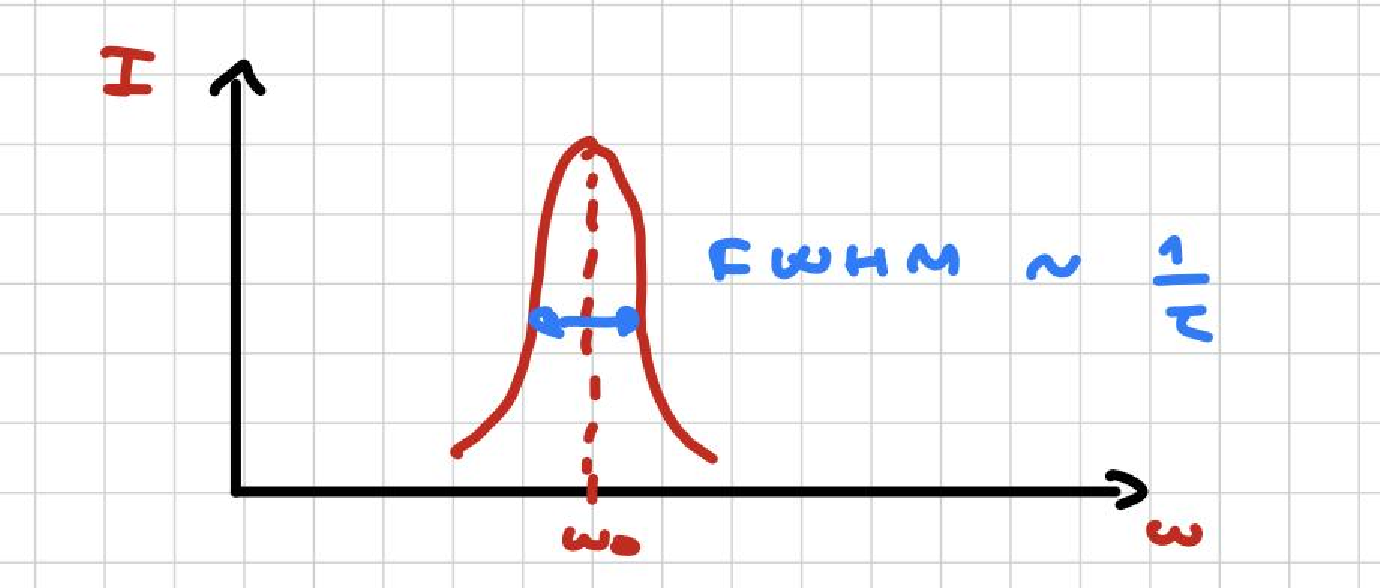
\includegraphics[width=0.8\linewidth]{images_in_pdf/6-/Grafico_23.pdf}
\end{figure}

The collision time $\tau_{\text{collision}}$ is typically shorter than the radiative lifetime, so the spectral width is mainly determined by collisions:
\[
\Delta\omega \approx \frac{1}{\tau_{\text{collision}}}
\]

Physically, this can be understood by noting that each atom emits a coherent wave only for a finite time between two successive collisions. Each collision interrupts the emission and randomizes the phase, so the emitted field can be seen as a sequence of short wave packets. According to Fourier analysis, a shorter emission time in the time domain corresponds to a broader distribution in frequency, which explains the increase in spectral width.

The coherence time is therefore limited by the same mechanism and is inversely related to the spectral width:
\[
\tau_c \approx \frac{1}{\Delta\omega}
\]

From a physical point of view, \hl{the coherence time represents the timescale over which the phase of the electromagnetic field remains correlated, i.e., how long the field \mbox{\say{remembers}} its phase}. Frequent collisions lead to rapid phase randomization and thus to a short coherence time.

In general, the \textbf{coherence time is determined by the spectral width and we can classify light with it}:
\begin{itemize}
    \item \textbf{Perfect monochromatic} source: $\Delta\omega=0$, which implies perfect phase correlation (ideal case, e.g. lasers), and therefore $\tau_c\to +\infty$.
    \item Thermal sources or \textbf{white light}: $\Delta\omega$ is broad, implying rapid phase fluctuations and therefore a very short coherence time.
\end{itemize}

\calloutinfo{For a \textbf{Doppler-broadened} source the frequencies of the emitted radiation are distributed according to a Gaussian function. This originates from the thermal motion of atoms: each atom moves with a different velocity and, due to the Doppler effect, emits radiation at a slightly shifted frequency. Since the \textbf{atomic velocities follow a Maxwell-Boltzmann distribution}, the resulting frequency distribution is Gaussian.}

\begin{figure}[H]
    \centering
    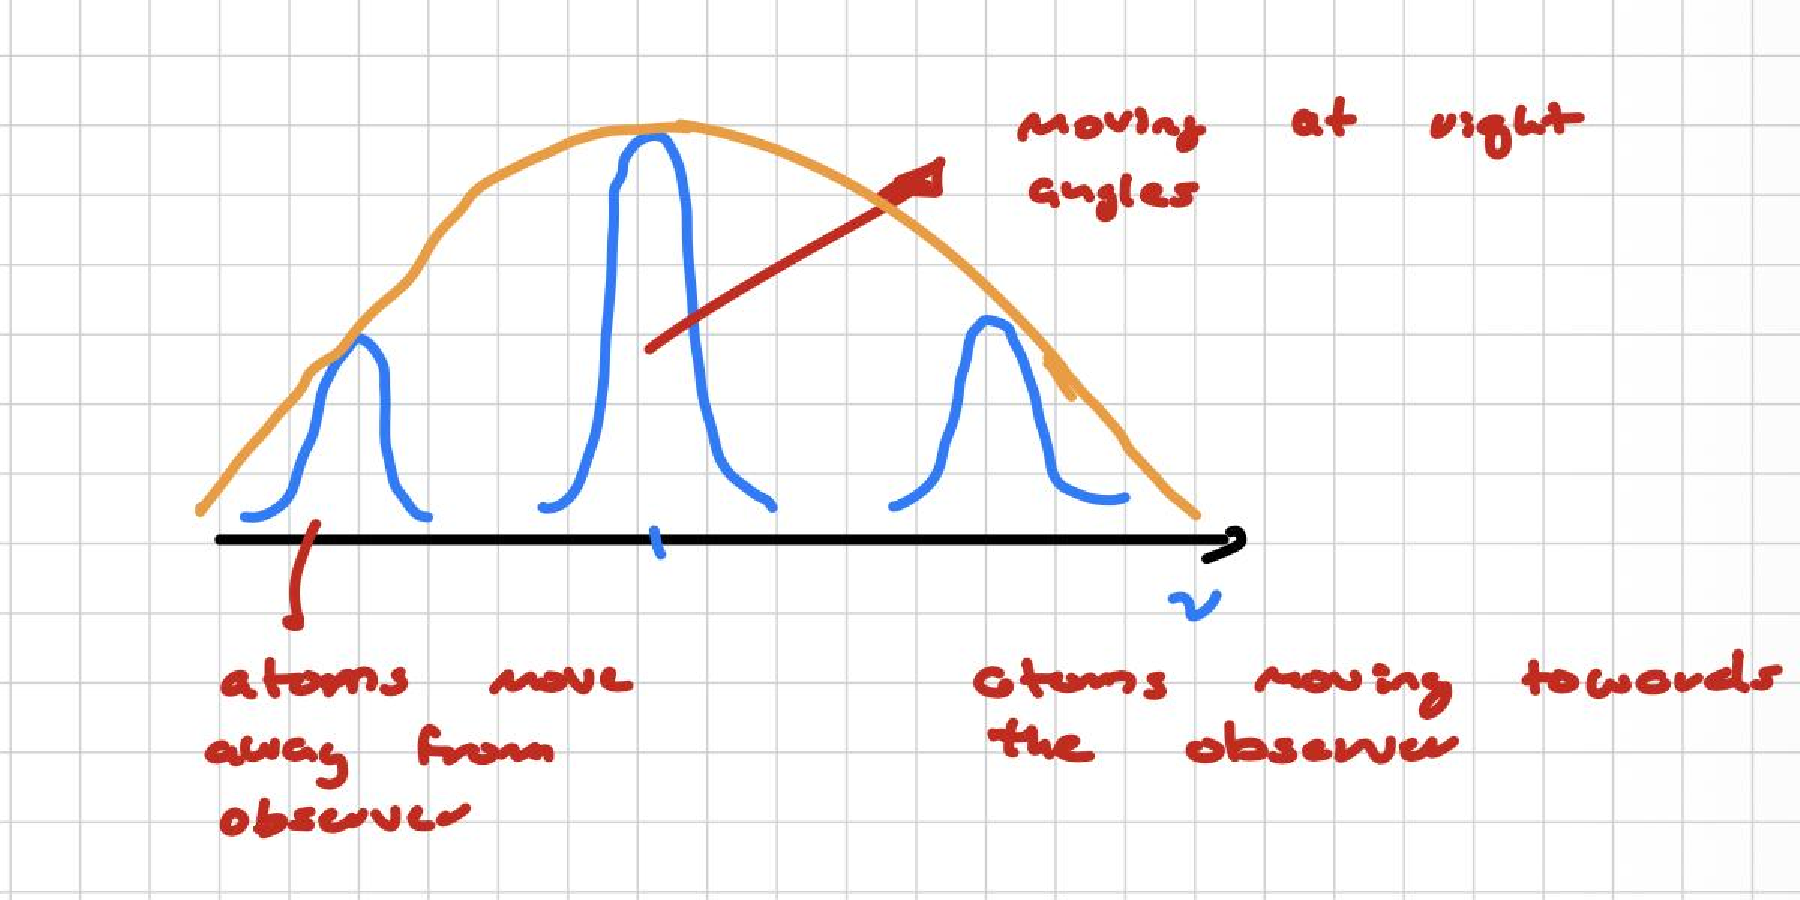
\includegraphics[width=0.8\linewidth]{images_in_pdf/6-/Grafico_24.pdf}
\end{figure}

Each individual atom is assumed to have a naturally broadened emission line, but random thermal motion shifts its central frequency due to the Doppler effect. It is therefore useful to distinguish between two broadening mechanisms:
\begin{itemize}
    \item \textbf{Homogeneous broadening:} \emph{all atoms are affected in the same way}. This is typically due to collision-induced phase interruptions and finite emission lifetime, and leads to a \textbf{Lorentzian line-shape}. It is fundamentally a temporal effect related to the finite coherence time of the emission process.
    \item \textbf{Inhomogeneous broadening:} \emph{different atoms are affected differently}. In this case, each atom emits at a slightly different frequency due to its velocity (Doppler effect), leading to a \textbf{Gaussian line-shape}. This is a statistical effect arising from the distribution of atomic velocities in the ensemble.
\end{itemize}

\subsection{Degree of first-order temporal coherence}

Suppose to come back on \textbf{Mach-Zehnder interferometer}:
\begin{itemize}
    \item We send a complex field $E(t)$ onto a beam splitter (BS), which divides the signal into two paths, $z_1$ and $z_2$ ($z_1 \neq z_2$). Each path contains a mirror and the two beams are then recombined by a second beam splitter, producing two output beams in the directions $E_3(t)$ and $E_4(t)$.
    \item The two beam splitters are identical and have the same \textbf{transmission} coefficient $\tran$ and \textbf{reflection} coefficient $\refl$ ($50{:}50$). These coefficients are also assumed to be independent of the frequency components of the light beam.
\end{itemize}
\begin{figure}[H]
    \centering
    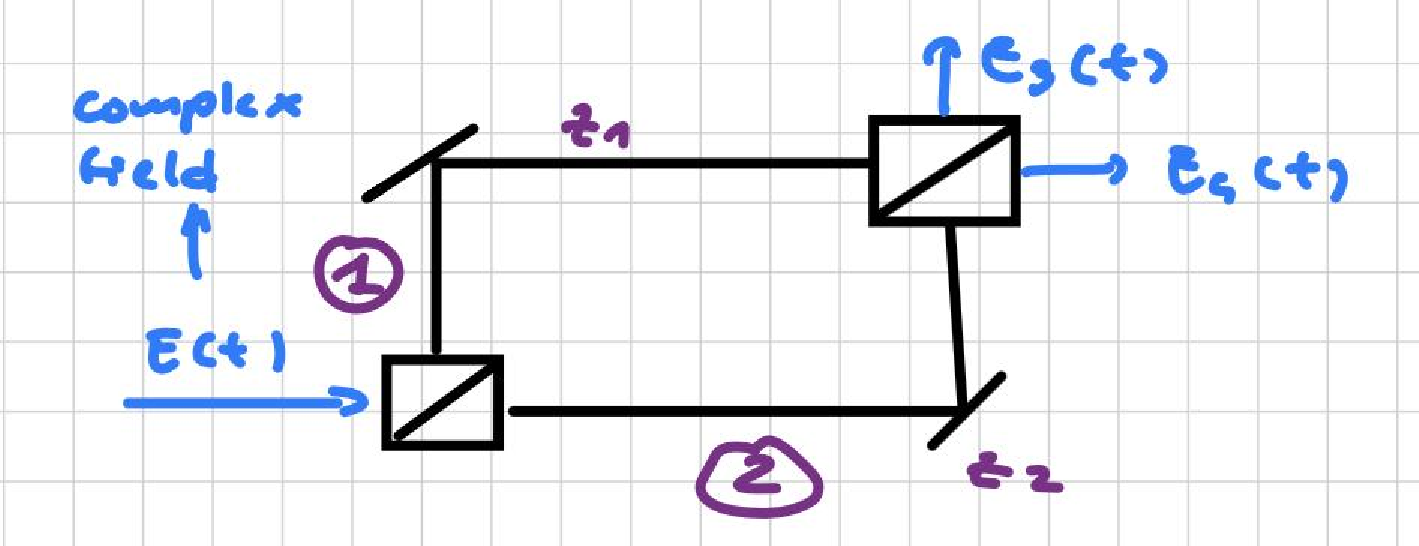
\includegraphics[width=0.8\linewidth]{images_in_pdf/6-/Grafico_25.pdf}
\end{figure}

Along the path $z_1$ we have $\Re[E(t)] = E_1(t)$, while along the path $z_2$ we have $\Re[E(t)] = E_2(t)$. The field reaches the second beam splitter with delays
\begin{equation}\label{eqn:6-delays}
    \Delta t_1 = \frac{z_1}{c}, \qquad \Delta t_2 = \frac{z_2}{c}
\end{equation}

if 
\[
t_1 = t - \frac{z_1}{c}, \qquad t_2 = t - \frac{z_2}{c}.
\]

then,
\begin{equation}\label{eqn:6-field-at-detector}
E_4(t) = \refl\, \tran\, E(t_1) + \tran\, \refl\, E(t_2).
\end{equation}

Averaging over a time window $T \gg \tau_c$, we obtain
\begin{equation}\label{eqn:6-intensity-at-detector}
I_4(t) = \frac{1}{2}\varepsilon_0 c\, \langle|E_4(t)|^2\rangle_T
= \frac{1}{2}\varepsilon_0 c\, |\refl|^2|\tran|^2
\left[
    \langle |E(t_1)|^2\rangle_T + \langle |E(t_2)|^2\rangle_T + 
    2\,\Re \langle E^*(t_1)E(t_2)\rangle_T
\right].
\end{equation}

Notice that the first two terms are the intensities produced by each path separately, in the absence of interference, while the \hl{last term is the interference contribution and is determined by the \textbf{first-order correlation function}}.
\begin{equation}\label{eqn:6-first-order-correlation-function}
\langle E^*(t_1)E(t_2)\rangle_T = \frac{1}{T}\int_T dt_1\,E^*(t_1)E(t_2).
\end{equation}

which is a function only of one variable, since this correlation depends only on the time difference, we define
\[
\tau = t_2 - t_1 = \textbf{fixed quantity},
\]

which means that it depends on the relative delay between the two arms.

If the physical mechanism responsible for the fluctuations does not change in time, then the statistical properties of the light are said to be \textbf{stationary}.
The quantity $\langle E^*(t_1)E(t_2)\rangle_T$ does not depend on the starting time of the averaging interval, provided that $T$ is much larger than the characteristic time of the fluctuations. Since the intensity is obtained by a statistical average over the field values at $t_1$ and $t_2$, the correlation function depends only on $\tau$ and can be written as
\[
\langle E^*(t_1)E(t_2)\rangle_T = \frac{1}{T}\int dt\,E^*(t)E(t+\tau).
\]

We can define the \textbf{degree of first-order temporal coherence} as:
\begin{equation}\label{eqn:6-degree-of-first-order-coherence}
g^{(1)}(\tau) = 
\frac{\langle E^*(t)E(t+\tau)\rangle}{\langle E^*(t)E(t)\rangle} \equiv
\frac{\langle E^*(t)E(t+\tau)\rangle}{\langle |E(t)|^2 \rangle}
\end{equation}

\textbf{which provides a direct measure of how much the electric field remains correlated with itself after a time delay $\tau$.}

Physically, $|g^{(1)}(\tau)|$ quantifies the ability of the field to produce interference: \hl{if $|g^{(1)}(\tau)| \approx 1$, the field is \textbf{highly coherent}} and stable in phase, whereas \hl{if $|g^{(1)}(\tau)| \to 0$}, the field has lost memory of its phase and \hl{\textbf{no interference} can be observed}.

\subsubsection{Correlation in a collision-broadened source}

If we assume a \emph{collision-broadened} light source, the electric field can be written as
\begin{equation}\label{eqn:6-collision-broadened-field}
E(t) = E_0 e^{-i(\omega_0 t + \phi(t))},
\end{equation}

where $E_0$ and $\omega_0$ are constant, while $\phi(t)$ undergoes random changes due to collisions. In this case,
\[
\langle E^*(t)E(t+\tau)\rangle
= E_0^2 e^{-i\omega_0 \tau}
\braket{\left[e^{-i\phi_1(t)} + \cdots + e^{-i\phi_n(t)}\right]
\left[e^{i\phi_1(t+\tau)} + \cdots + e^{i\phi_n(t+\tau)}\right]}.
\]

The \hl{phase angles} associated with different atoms are statistically independent and randomly distributed; therefore, all cross terms \hl{vanish upon averaging}. As a result,
\[
\langle E^*(t)E(t+\tau)\rangle
= E_0^2 e^{-i\omega_0 \tau}\sum_{i=1}^{n} \braket{e^{i[\phi_i(t+\tau)-\phi_i(t)]}}
= n \cdot \langle E_i^*(t)E_i(t+\tau)\rangle.
\]

\calloutinfo{This shows that the total correlation function is entirely determined by the contribution of individual atoms. Physically, this means that coherence is preserved only as long as each atom maintains a well-defined phase during its emission.
After an atom undergoes a collision, its phase is randomized, effectively resetting its contribution to the field. Therefore, the single-atom correlation function is non-zero only if no collision occurs within the time interval $\tau$. In other words, it is \textbf{proportional to the probability that the atom remains in free flight for a time longer than $\tau$.}}

From the kinetic theory of gases, the time between collisions follows an exponential distribution:
\[
\rho(\tau')\,d\tau' = \frac{1}{\tau_0}e^{-\frac{\tau'}{\tau_0}}d\tau',
\]

where $\tau_0$ is the average time between collisions, here $\tau_0=\tau_c$. The probability that no collision occurs in a time interval $\tau$ is then
\[
\int_{\tau}^{\infty} d\tau'\,\rho(\tau') = e^{-\frac{\tau}{\tau_0}}.
\]

As a consequence,
\[
\langle E^*(t)E(t+\tau)\rangle
= E_0^2 e^{-i\omega_0 \tau-\frac{\tau}{\tau_0}},
\]

which shows that the \hl{field loses phase memory exponentially in time}. Finally, the degree of coherence (Eqn.~\ref{eqn:6-degree-of-first-order-coherence}) becomes
\begin{equation}\label{eqn:6-g1-collision-broadened}
g^{(1)}(\tau)
= e^{-i\omega_0 \tau-\frac{|\tau|}{\tau_c}},
\end{equation}

where $\tau_c$ defines the coherence time, i.e. the characteristic time over which the phase of the field remains correlated. This exponential decay directly explains the progressive loss of interference visibility as the time delay between the two paths increases.
\begin{figure}[H]
    \centering
    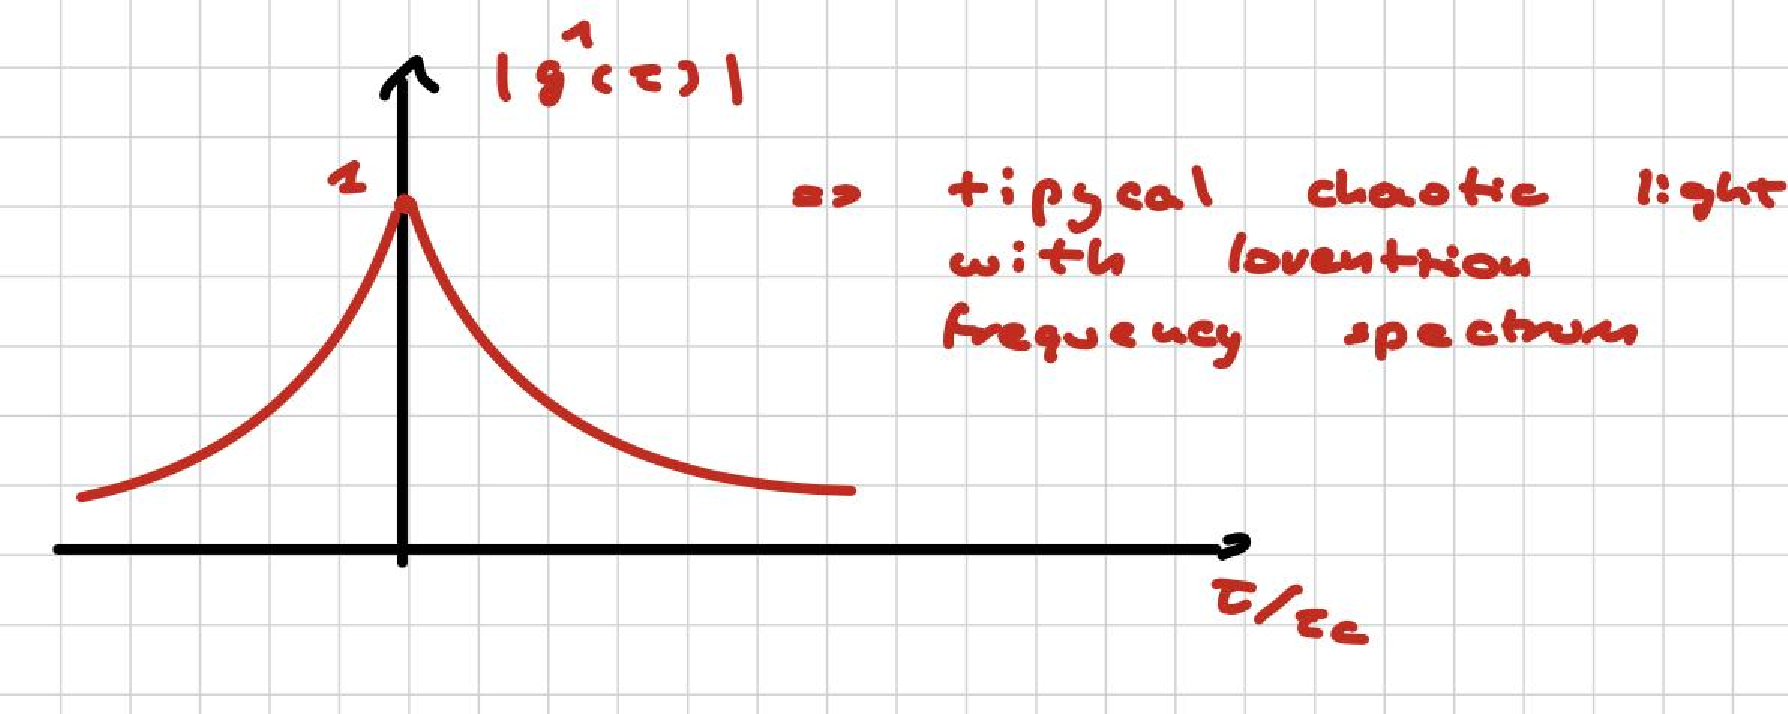
\includegraphics[width=0.8\linewidth]{images_in_pdf/6-/Grafico_26.pdf}
\end{figure}

\subsubsection{Correlation in a Doppler-broadened source}

Similarly, it can be shown that for a \emph{Doppler-broadened} source:
\begin{equation}\label{eqn:6-g1-doppler-broadened}
g^{(1)}(\tau) 
= e^{-i\omega_0\tau-\frac{\pi}{2}\frac{\tau^2}{\tau_c^2}}
\end{equation}
\begin{figure}[H]
    \centering
    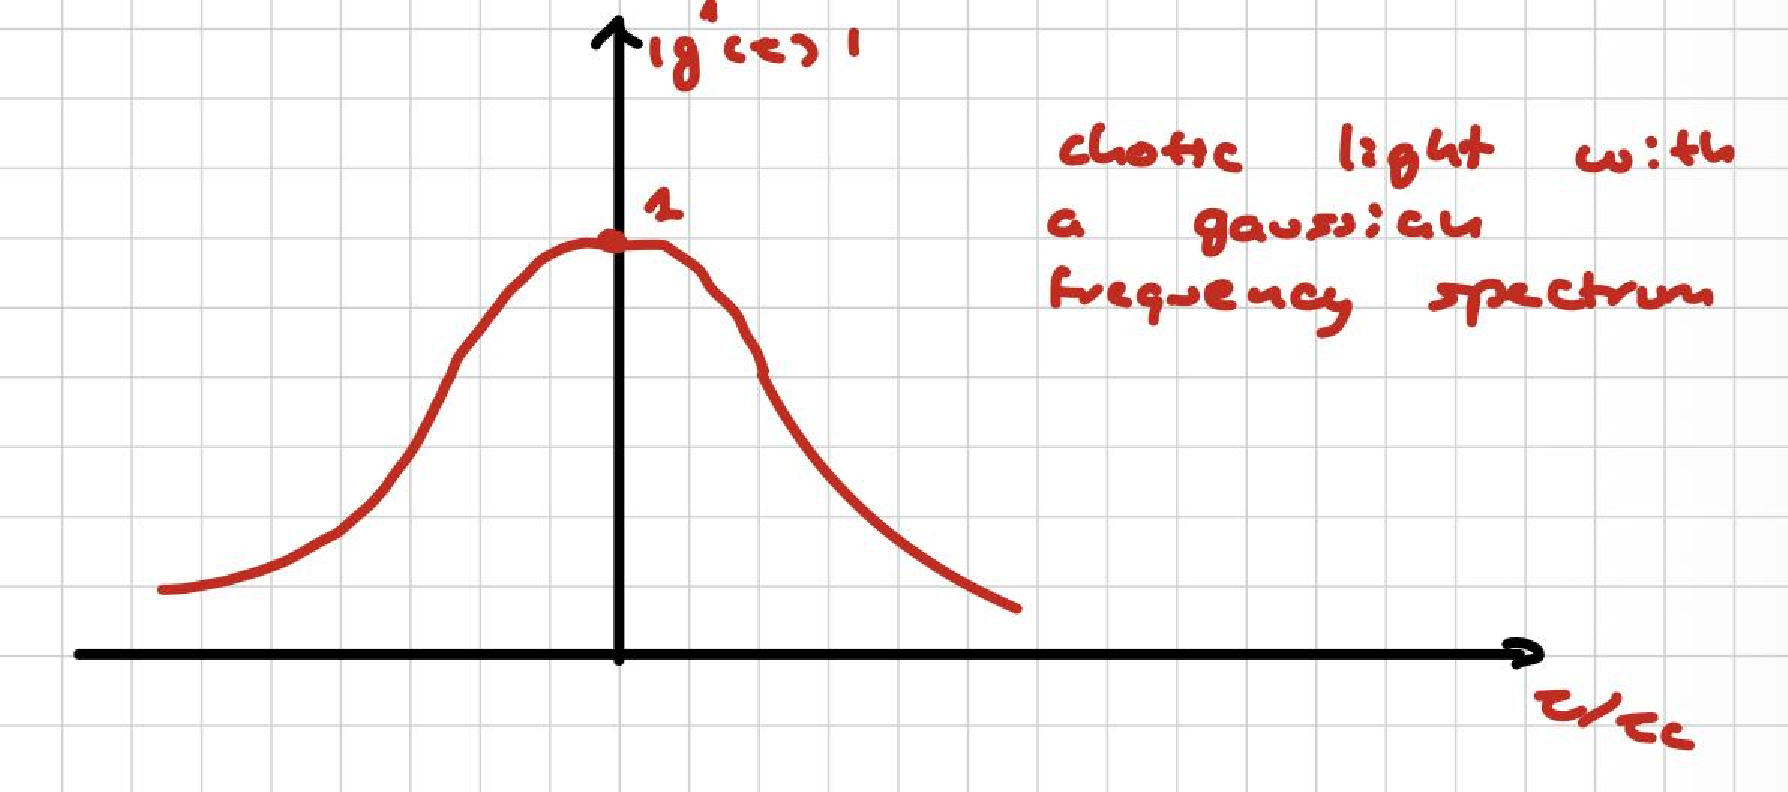
\includegraphics[width=0.8\linewidth]{images_in_pdf/6-/Grafico_27.pdf}
\end{figure}

Observe that:
\begin{itemize}
    \item $g^{(1)}(0)=1$;
    \item light remains first-order coherent for time delays such that $|\tau| \ll \tau_c$.
\end{itemize}

When the delay becomes much larger than the coherence time, the correlation between the fields at $t$ and $t+\tau$ is lost and
\[
\langle E^*(t)E(t+\tau)\rangle \to 0,
\]

so that
\[
g^{(1)}(\tau)\to 0.
\]

\question{What happens if we consider a classical wave with stable amplitude and phase?}{%
\[
E(t)=E_0 e^{-i\omega_0 t+i\phi},
\]

where $\phi$ and $E_0$ are fixed quantities. In this case,
\[
g^{(1)}(\tau)=e^{-i\omega_0\tau}\cdot \langle e^{i[\phi(t+\tau)-\phi(t)]}\rangle.
\]

The first factor is the rapidly oscillating optical phase, with period
\[
T=\frac{2\pi}{\omega_0},
\]

and it gives rise to the interference fringes in the Mach-Zehnder interferometer, while the bracket term contains the coherence information.

For a perfectly coherent light source,
\[
\tau_c\to\infty,
\]

which means that the phase remains correlated for any finite delay. In this ideal case,
\[
|g^{(1)}(\tau)|=1
\]

for all $\tau$.
}

\subsubsection{Correlation in our MZI example}

If we come back on M.Z. interferometer, where we stopped at Equation~\ref{eqn:6-intensity-at-detector}, and average the intensity over a time interval $T$, we obtain:
\[
\begin{split}
    \langle I_4(t)\rangle_T &= 
    \frac{1}{2}\varepsilon_0c\, |\refl|^2|\tran|^2\ 
    \biggl[
        \langle |E(t_1)|^2\rangle_T + \langle |E(t_2)|^2\rangle_T + 
        2\,\Re \langle E^*(t_1)E(t_2)\rangle_T
    \biggr] =\\[0.75ex]
    &= \frac{1}{2}\varepsilon_0c\, |\refl|^2|\tran|^2\ 
    \langle |E(t)|^2\rangle\,
    \left[2+2\,\Re\frac{\langle E^*(t_1)E(t_2)\rangle}{\langle |E(t)|^2\rangle}\right]
\end{split}
\]  

where we have used the fact that the time average of the intensity is the same at $t_1$ and $t_2$ because of stationarity
\begin{equation*}
|E(t_1)| = |E(t_2)| \hspace{0.2cm}\text{through a 50:50 B.S.}
\end{equation*}
finally:
\begin{equation}\label{eqn:6-intensity-at-detector-final}
\langle I_4(t)\rangle_T =
 2\ |\refl|^2|\tran|^2\ \langle I(t)\rangle\,
\left[
    1+\Re\bigl(g^{(1)}(\tau)\bigr)
\right]
\end{equation}

The output intensity is therefore proportional to $\langle I(t)\rangle$ and modulated by the factor $1+\Re(g^{(1)}(\tau))$.

The fringe visibility is given by
\[
V=|g^{(1)}(\tau)|=\frac{I^{\max}-I^{\min}}{I^{\max}+I^{\min}}.
\]

As we've seen in Eqn.~\ref{eqn:6-g1-collision-broadened}, for chaotic light with Lorentzian broadening,
\[
g^{(1)}(\tau)=e^{-i\omega_0\tau-\frac{|\tau|}{\tau_c}},
\]

so that
\[
\langle I_4(t)\rangle=2\, |\refl|^2|\tran|^2\ \langle I(t)\rangle\,
\left[
    1+e^{-\frac{|\tau|}{\tau_c}}\cos(\omega_0\tau)
\right].
\]

This means that when $|\tau|\gg\tau_c$, the fringes disappear.

In conclusion, the first-order temporal coherence and the frequency spectrum are directly related, and they both determine the visibility of interference in optical experiments.

\begin{table}[H]
\label{tab:type-of-light}
\centering
\begin{tabular}{|c|c|c|c|c|}
\hline
Type of light & $\Delta \omega$ & Coherence & $\tau_c$ & $g^{(1)}(\tau_c)$ \\
\hline
Monochromatic & 0 & Perfect & $+\infty$ & 1 \\
\hline
Chaotic & $\Delta \omega$ & Partial & $\sim \frac{1}{\Delta \omega}$ & $0<|g^{(1)}|<1$ \\
\hline
Incoherent & $\infty$ & None & 0 & 0 \\
\hline
\end{tabular}
\end{table}